%MEJORAS PROPIAS AL ALGORITMO DE PAGERANK
\subsubsection{Mejoras a PageRank - Peso a los enlaces}

La idea detrás de PageRank es que las "buenas" páginas hacen referencia a otras "buenas" páginas. Por lo tanto, las páginas a las que hacen referencia esas "buenas" páginas tienen un PageRank más alto. Suponiendo que un usuario navega por la Web de forma aleatoria, de modo que, si está en una página, con cierta probabilidad se aburre y abandona la página, o elige de manera uniforme y aleatoria seguir uno de los enlaces de la misma página en la que se encuentra (eliminando los autoenlaces). Por lo tanto, la probabilidad de estar en la página "p" es

\begin{equation} 
	\label{eqn:ecuacionWLRank1} 
	PR(p) = \frac{q}{T} + (1 - q) \sum_{i} \frac{PR(r_i)}{L(r_i)} 
\end{equation}

donde $T$ es el número total de páginas, $q$ es la probabilidad de salir de la página $p$ (en el trabajo original de PageRank se sugiere $q = 0:15$), $ri$ son las páginas que apuntan a la página $p$, y $L(ri)$ es el número de enlaces en la página $ri$. Estos valores se pueden usar como clasificación de páginas y se pueden calcular mediante un algoritmo iterativo que converge bastante rápido, ya que estamos interesados en el orden de clasificación en lugar de los valores reales. El término $q$ se denomina factor de amortiguamiento, ya que disminuye exponencialmente el spam de enlaces basado en secuencias de enlaces que regresan a una página.

De aquí surge una variante al algoritmo de PageRank original de Google, llamada WLRank propuesta en el trabajo de Ri Baeza-Yates y Emilio Davies \cite{baeza2004web}.

WLRank (Weighted Links Rank) asigna el valor de clasificación $R(i)$ a la página $i$ usando las siguientes ecuaciones:

\begin{equation} 
	\label{eqn:ecuacionWLRank2} 
	R(i) = \frac{q}{T} + (1 - q) \sum_{j} \frac{W(j,i)R(j)}{\sum_{k}W(j,k)} 
\end{equation}

\begin{equation} 
	\label{eqn:ecuacionWLRank3} 
	W(j,i) = L(j,i)(c+T(j,i)+AL(j,i)+RP(j,i))
\end{equation}

donde dado un enlace de la página $j$ a la página $i$ se tiene:

$L(j; i)$ es $1$ si el enlace existe, o $0$ en caso contrario, y c es una constante que da un peso base a cada enlace,
$T(j; i)$ es un valor que depende de la etiqueta donde se inserta el enlace,
$AL(j;i)$ es la longitud del texto "ancla" del enlace dividida por una constante d que depende que estima la longitud promedio del texto ancla en caracteres, y $RP(j;i)$ es la posición relativa del enlace en la página ponderado por una constante b.

Al igual que en PageRank, $R(i)$ corresponde a la probabilidad de llegar a la página $i$ mientras navega por la Web. Si $W(j; i) = L(j; i)$ tenemos el PageRank original. Los cambios se explican a continuación. El término $T(j; i)$ es una secuencia de constantes dependiendo de la etiqueta donde se encuentre el enlace. Por ejemplo, si el enlace está dentro de una etiqueta $<h1>$, tendrá un valor alto de $T(j; i)$, un poco menos para $<h2>$, etc. Lo mismo para otras etiquetas de énfasis como $<strong>$ o $<b>$ .

El término $AL(j;i)$ da más valor a los enlaces en los que el creador explica con más detalle a qué recurso Web se está enlazando. Por ejemplo, esto le da menos peso a los enlaces descritos con home o aquí. Finalmente, el término $RP(j; i)$ da más peso a los enlaces que están al principio de la página que al final de la página (físicamente en el código HTML, no necesariamente en la vista del navegador).

Gracias a esta mejora sobre la fórmula original de PageRank es posible entonces darle mayor consideración en la fórmula a aquellos enlaces que tienen más pesos que otros.

Se procedió a adecuar nuestra fórmula de modo de contemplar los pesos en los enlaces y de esta forma realizar ciertas pruebas simples que comprueben que la modificación realizada consigue ajustar a nuestro modelo en una mejora respecto al algoritmo de PageRank original.

A continuación se muestra el ejemplo de 6 nodos mostrado con anterioridad en donde se puede observar el resultado ponderando los enlaces.

\begin{figure}
	\centering
	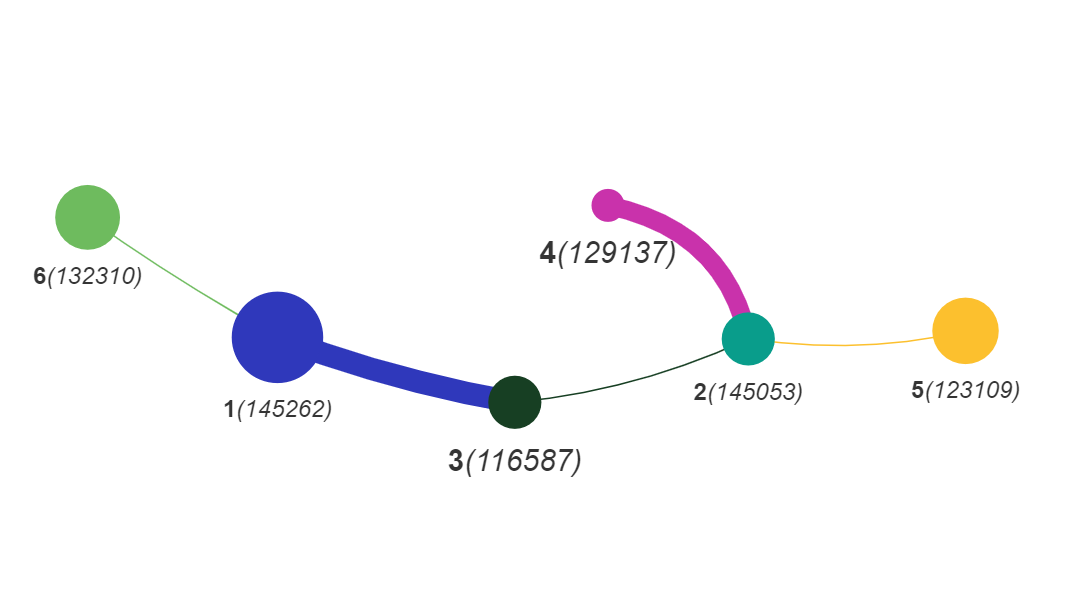
\includegraphics[width=0.50\linewidth]{6nodos-pageRank-peso-enlaces.png}
	\caption{Resultado de ejecución de PageRank para 6 nodos con modificación WLRank.} 
	\label{fig:6nodos-pageRank-peso-enlaces}
\end{figure}

Se puede apreciar a simple vista que ahora al tener peso las relaciones en la fórmula el resultado es mucho más preciso, existen muchos casos en cómun entre $145262$ y $116587$, lo que justifica la modificación en el ranking general. El nodo $145262$ tiene $1$ caso en cómún con $132310$ y $18$ con $116587$, un total de $19$ relaciones a ese nodo. Por otra parte el nodo que quedó en segunda posición en el ranking ($145053$), tiene un total de $15$ enlaces provenientes de $13$ casos en común con el nodo $129137$ y de $1$ caso en cómun con el nodo $116587$ y con el nodo $123109$.

\subsubsection{Mejoras a PageRank - Peso a los nodos}

Como se mencionó en el punto anterior, el algoritmo de PageRank en su versión original, no hace valorar al peso de los enlaces (tema propuesto y resuelto con anterioridad), ni el peso de los nodos. Este último es otro punto muy importante a la hora de evaluar a los individuos en los grafos resultantes, como así también a la hora del posible descubrimiento de una supuesta banda delictiva.

Es casi imposible evaluar y calificar de banda delictiva a individuos que tengan un bajo grado de relación entre sí, y que además cada uno tenga como antecedente penal un número pequeño de casos en su haber.

Para ello, se procedió del mismo modo que con los pesos en los enlaces, a modificar la fórmula original de PageRank en pos de obtener un resultado más significativo y darle más importancia en el grafo a aquellos nodos que tengan más casos (más tamaño en el grafo), cuando se encuentren relacionados con otros con la misma cantidad de relaciones. El objetivo principal de dicha modificación es generar un desempate de valor de ranking para aquellos nodos que en el algoritmo original de pagerank obtengan igual puntaje. Ante una situación de igualdad de ranking, el nodo que tenga un mayor tamaño quedará con un mayor valor ponderado.

No se encontró bibliografía dedicada que aporte datos para aplicar a la fórmula, por lo que se realizó  en base a lo ya estudiado una modificación propia. 

Para comenzar con la ponderación del peso de los nodos, se identifica primero al nodo con mayor peso en el grafo, y luego sobre el resultado de la fórmula de PageRank se procede a sumar un nuevo valor empírico que surge de dividir el tamaño de cada nodo por el tamaño de mayor peso ya calculado, para luego multiplicarlo por el valor de PageRank anteriormente calculado. Cada nuevo valor de ranking sobre cada nodo es sobreescrito y pasa a ser el valor final. A continuación se detalla el algoritmo SQL de actualización.

\begin{scriptsize}{1}
	\tiny{
		\begin{verbatim}
			DECLARE @NodeMax float
			SELECT @NodeMax = MAX(n.nodeValue) FROM #Node n			
			IF(@pesoEnNodos = 1)
			BEGIN
			UPDATE PR 
			SET rank = rank + ( (#Node.nodeValue/@NodeMax) * rank )
			FROM #PageRank PR
			INNER JOIN #Node ON PR.id = #Node.id
			end
		\end{verbatim}
	}
\end{scriptsize}


En donde $Node$ es la tabla de los Nodos, $nodeValue$ es el peso de cada nodo, $NodeMax$ se obtiene como el máximo valor de peso de la tabla de Nodos, y $rank$ es el valor previo de PageRank. Al realizar el $SET$ se produce la actualización de cada Ranking para cada nodo. 

A continuación se muestra el mismo ejemplo de 6 nodos mostrado con anterioridad en donde se puede observar el resultado ponderando sólo los nodos.

\begin{figure}
	\centering
	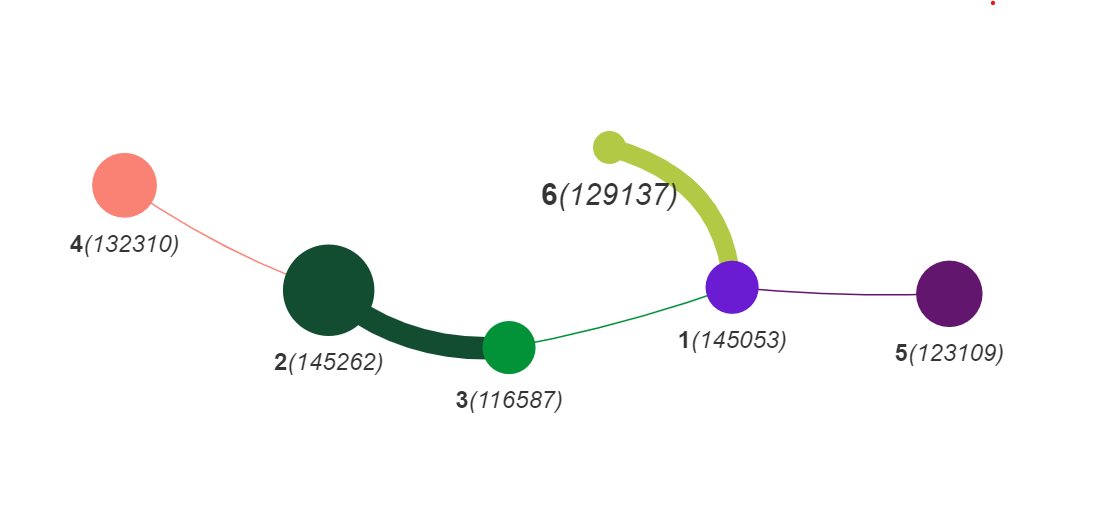
\includegraphics[width=0.50\linewidth]{6nodos-pageRank-peso-nodos.png}
	\caption{Resultado de ejecución de PageRank para 6 nodos con modificación en peso de Nodos.} 
	\label{fig:6nodos-pageRank-peso-nodos}
\end{figure}

En el mismo es posible observar comparando la ejecución de PageRank, que mantiene el resultado principal de la fórmula original, pero para los casos de nodos con "empate" de ranking, ahora ponderará con mayor valor al que posea un peso mayor. Los nodos $129137$ y $123109$ que en el algortimo original compartían el quinto lugar en el ranking, ahora pueden diferenciarse por su tamaño (cantidad de casos penales de cada persona). El nodo $123109$ posee $68 casos penales$ asociados, quedando en quinto lugar, mientras que el nodo $129137$ se encuentra vinculado a $47 casos penales$, por lo que queda relegado al sexto lugar en el ranking de este grafo.

Por último se muestra el mismo ejemplo, pero ahora con ambas modificaciones aplicadas a la fórmula original de PageRank.

\begin{figure}
	\centering
	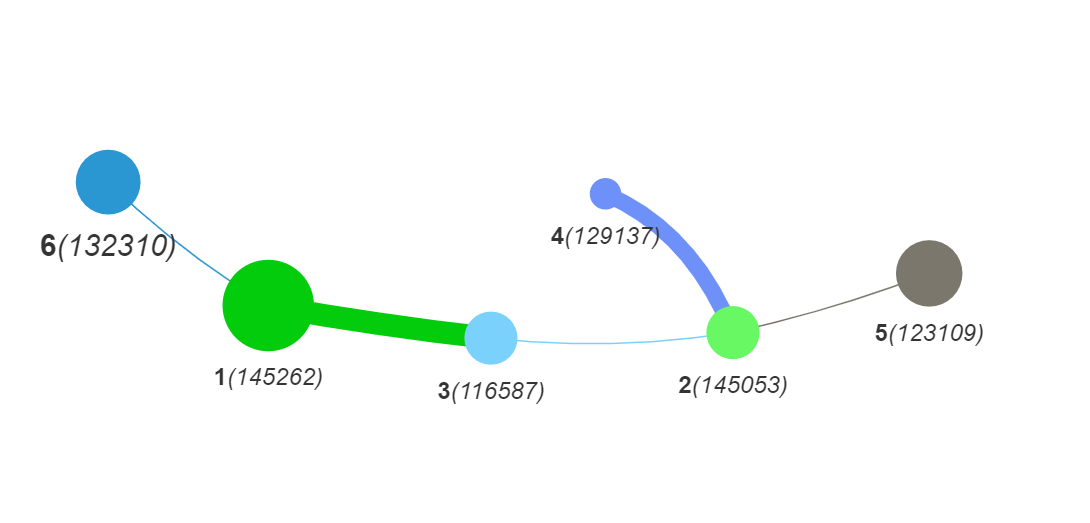
\includegraphics[width=0.50\linewidth]{6nodos-pageRank-peso-nodos-enlaces.png}
	\caption{Resultado de ejecución de PageRank para 6 nodos con modificación WLRank y la modificación propia en peso de Nodos.} 
	\label{fig:6nodos-pageRank-peso-nodos-enlaces}
\end{figure}

